% DRAFT 2026-09-27 (agent-written; the author is the verification loop).
% Every number is a macro from numbers.tex, generated by make_numbers.py.
% Target: J. Rheol. short communication.
\documentclass[aps,pre,reprint,superscriptaddress,nofootinbib]{revtex4-2}
\usepackage{amsmath,graphicx,siunitx}
% generated by make_numbers.py; do not edit
\newcommand{\allHiPm}{1.64}
\newcommand{\allHiSi}{1.59}
\newcommand{\allLoPm}{0.71}
\newcommand{\allLoSi}{0.54}
\newcommand{\ctlDiffPct}{41}
\newcommand{\ctlDirect}{0.289}
\newcommand{\ctlInverted}{0.488}
\newcommand{\depthHiPm}{0.64}
\newcommand{\depthHiSi}{0.74}
\newcommand{\depthLoPm}{0.56}
\newcommand{\depthLoSi}{0.65}
\newcommand{\floorPm}{19.66}
\newcommand{\floorSi}{6.62}
\newcommand{\fullFallSi}{2.00}
\newcommand{\fullHiPm}{1.09}
\newcommand{\fullHiSi}{1.09}
\newcommand{\fullLoPm}{0.88}
\newcommand{\fullLoSi}{0.54}
\newcommand{\gFiftyHiPm}{1.64}
\newcommand{\gFiftyHiSi}{1.59}
\newcommand{\gFiftyLoPm}{1.41}
\newcommand{\gFiftyLoSi}{0.74}
\newcommand{\gFiftySpreadPm}{1.16}
\newcommand{\gFiftySpreadSi}{2.14}
\newcommand{\minOverSolver}{2.7}
\newcommand{\nDepthPm}{3}
\newcommand{\nDepthSi}{4}
\newcommand{\nRatesPm}{3}
\newcommand{\nRatesSi}{4}
\newcommand{\phiPm}{0.496}
\newcommand{\phiSi}{0.391}
\newcommand{\phimPm}{0.587}
\newcommand{\phimSi}{0.508}
\newcommand{\rateSpanPm}{10}
\newcommand{\rateSpanSi}{10}
\newcommand{\solverGammaZero}{0.2}
\newcommand{\sweepMinPm}{19.47}
\newcommand{\sweepMinSi}{6.44}
\newcommand{\tFiftySpreadPm}{11.6}
\newcommand{\tFiftySpreadSi}{21.4}


\begin{document}

\title{The Wyart--Cates strain clock depends on the protocol:\\ shear reversal gives order one}

\author{[AUTHOR --- to be confirmed]}
\affiliation{[AFFILIATION --- to be confirmed]}

\date{\today}

\begin{abstract}
Continuum models of shear-thickening suspensions let the frictional contact fraction $f$
relax toward its steady value over a strain $\gamma_0$. The values in use span an order
of magnitude, from $0.023$ in particle simulations of a stress step to $\approx 0.2$ in
start-up experiments on corn starch, and nobody has measured $\gamma_0$ from a flow reversal,
although reversal is the protocol through which $\gamma_0$ has been defined. We read
$\gamma_0$ from the published shear-reversal transients of \citet{Lin2015} on two
colloidal suspensions. We first show that the inversion of the Wyart--Cates viscosity
for $f$ is affine in $\phi_J/\phi$. Consequently a relaxation constant fitted with free
amplitudes is independent of $\phi$, $\phi_0$ and $\phi_m$, even though a flow curve
cannot determine $\phi_m$, and it depends only on the divergence exponent. The fitted
clock is $\fullLoSi$--$\fullHiSi$ on $2\,\mu$m silica and $\fullLoPm$--$\fullHiPm$ on
$1.4\,\mu$m PMMA. It is controlled by strain rather than time over a decade in rate, and
on silica it \emph{falls} with rate, which a relaxation law with an added time term
cannot produce. The minimum just after reversal lies at $\depthLoPm$--$\depthHiSi$ of the model's own
frictionless floor, which is itself within $3\%$ of the lowest steady-state viscosity of  % 3%: numbers.tex floorSi/sweepMinSi = 1.028, floorPm/sweepMinPm = 1.010
each sample. On the one record where contact stress is known directly, a simulation,
the directly evaluated contact-stress fraction recovers $\ctlDiffPct\%$ faster than the
inverted $f$. On a second silica, constant-stress start-up shows no exponential clock at all: the viscosity rises abruptly after a strain of $\suJamLo$--$\suJamHi$, partly coupled to the instrument. We argue that $\gamma_0$ is not a material constant of scalar Wyart--Cates
models: it depends on the protocol and on the definition of $f$.
\end{abstract}

\maketitle

\section{Introduction}

The Wyart--Cates (WC) model~\cite{WyartCates2014} describes discontinuous shear thickening
(DST) through a fraction $f$ of frictional contacts that interpolates the jamming volume
fraction $\phi_J=(1-f)\phi_0+f\phi_m$ between its frictionless and frictional values.
Unsteady flows need a law for how $f$ evolves. The common choice is a first-order relaxation
in strain, sometimes with an additional time term~\cite{Mari2015,Chacko2018,Richards2019}:
\begin{equation}
\frac{df}{dt}=-\left(\frac{\dot\gamma}{\gamma_0}+\frac{1}{t_r}\right)\left(f-f_{ss}\right).
\label{eq:relax}
\end{equation}
At steady state $f=f_{ss}$ whatever $\gamma_0$ is, so a flow curve carries no information about the clock.
The values in use differ by an order of magnitude. Particle simulations of a stress step
gave an exponential strain scale of $0.023$~\cite{Mari2015}, which Chacko \emph{et al.}\
adopt~\cite{Chacko2018}. The same paper defines $\gamma_0$ as ``of order the strain required
to evolve from one steady-state to another (for instance on flow reversal)''.
\citet{Richards2019} report $\gamma_0=O(10^{-1})$ from imposed-rate experiments.
Corn-starch shear fronts give $\gamma^*\approx0.197$~\cite{Han2018}, a start-up scale in a different, multiplicative closure $g=1-e^{-\gamma/\gamma^*}$ rather than the constant of Eq.~(\ref{eq:relax}), and
linear-stability work sweeps $0.05$--$0.5$~\cite{DarboisTexier2023}.
Reversal recovery is known to take a strain ``of order unity''~\cite{Lin2015,NessSun2016}.
Gillissen \emph{et al.}\ fitted the structural strain scale of a tensorial model to
simulated reversal~\cite{Gillissen2019}. No value of the scalar clock in
Eq.~(\ref{eq:relax}) has been measured from an experimental reversal.

Reversal has a subtlety that should be stated first. In scalar WC, $f_{ss}$ depends on
$|\sigma|$ alone, so reversing the flow at constant rate leaves $f=f_{ss}$ and
Eq.~(\ref{eq:relax}) predicts \emph{no} transient. Reading $\gamma_0$ off a reversal
therefore assumes that reversal resets $f$, and it tests only the \emph{recovery} half of
the law. That is the physical reason a fabric is needed~\cite{Gillissen2019}. It is also what
the clock in every reversal-based estimate means, ours included.

\section{Data and inversion}

We use the deposited data of \citet{Lin2015} (Edinburgh DataShare 10283/886): the relative
viscosity $\eta_r$ against accumulated strain after a reversal, at four shear rates each
for $2\,\mu$m silica (their Fig.~2b) and $1.4\,\mu$m PMMA (Fig.~2d), and the steady rate
sweep of the same samples (Figs.~2a,c). The records are uniformly sampled in strain up
to $\gamma=10$ ($10^4$--$2.5\times10^4$ points each).

\emph{Steady fit.} We fit $\eta_r=(1-\phi/\phi_J)^{-n}$ with
$f_{ss}=\exp(-\sigma^*/\sigma)$ to the thickening branch of each sweep, with $n=2$ and
$\phi_0$ fixed at $0.64$. A single flow curve determines only the ratios
$\phi/\phi_0$ and $\phi_m/\phi$ (the model is homogeneous of degree zero in
$(\phi,\phi_0,\phi_m)$), so $\phi_0$ is a gauge choice and nothing below depends on it.
The fits give $\phi=\phiSi$, $\phi_m=\phimSi$ (silica) and $\phi=\phiPm$, $\phi_m=\phimPm$
(PMMA) in that gauge.

\emph{The inversion is affine.} Write $u=\phi_J/\phi=1/(1-\eta_r^{-1/n})$. Solving
$\phi_J=(1-f)\phi_0+f\phi_m$ for $f$ gives
\begin{equation}
f=A+Bu,\qquad A=\frac{\phi_0/\phi}{\phi_0/\phi-\phi_m/\phi},\quad
B=\frac{-1}{\phi_0/\phi-\phi_m/\phi}.
\end{equation}
For any packing triple, $f(\gamma)$ is an affine image of $u(\gamma)$, and $u$ depends only on
the data and $n$. A relaxation $f=f_{ss}+(f_0-f_{ss})e^{-\gamma/\gamma_0}$ fitted with both
amplitudes free is exactly invariant under affine maps of the ordinate, so $\gamma_0$ is
independent of $\phi$, $\phi_0$ and $\phi_m$ jointly. We checked this at four triples far
off the covariance ray, with $\phi/\phi_0$ from $0.32$ to $0.87$: the fitted clocks are
bit-identical. Across $n=1.8$--$2.5$ they move by at most $1.8\%$. The clock therefore  % 1.8%: scripts/gate_g11.py G11a-ii 'worst 1.80%'
escapes the degeneracy that makes $\phi_m$ unidentifiable from one flow curve.

\emph{Fit.} Each record is reduced to log-spaced bins, each holding the median and the
within-bin scatter. We start at the binned reversal minimum, eliminate the two amplitudes
exactly by weighted linear least squares, and scan $\gamma_0$ on a logarithmic grid
(variable projection~\cite{GolubPereyra1973}). A general-purpose nonlinear optimiser on the same records returned values differing by
more than an order of magnitude depending only on its convergence tolerance
(	exttt{src/dst\_fit/transient.py}, 	exttt{fit\_recovery} docstring). We also report a
fit-free landmark, $\gamma_{50}$: the strain from the minimum to half the plateau in $f$.
Its definition does not depend on any fit window.

\emph{Where the fit starts.} The minimum is a broad, noisy trough, so its position is uncertain by $\sim0.1$--$0.2$ in strain. A delay measured from it is ill-posed; our attempt to measure one failed its own synthetic controls (\texttt{scripts/probe\_rebuild\_lag.py}). Moving the start anywhere up to $\startShiftRange$ strain \emph{after} the minimum changes the fitted clock by at most $\startShiftWorst\times$ on every record. Starting \emph{before} the minimum brings in the still-falling viscosity, which Eq.~(\ref{eq:relax}) does not describe. There the fit is ill-posed: on silica at $5$\,s$^{-1}$ it has no interior optimum (\texttt{scripts/probe\_start\_sensitivity.py}).

\section{Results}

\emph{The reversal minimum lies below the model's frictionless floor.}
With $f\ge0$, WC bounds the viscosity from below by $(1-\phi/\phi_0)^{-n}$:
$\floorSi$ for silica and $\floorPm$ for PMMA. Figure~\ref{fig:reversal}(a,b) shows
the smoothed post-reversal minima at $\depthLoSi$--$\depthHiSi$ (silica,
$\nDepthSi$ rates) and $\depthLoPm$--$\depthHiPm$ (PMMA, $\nDepthPm$ rates) of this floor.
The fourth PMMA record ($\dot\gamma=0.05$\,s$^{-1}$) stays below the floor throughout. The floor is not an artefact of the fit. It lies within $3\%$  % 3%: numbers.tex floorSi/sweepMinSi = 1.028, floorPm/sweepMinPm = 1.010
of the lowest viscosity on each sample's own steady sweep ($\sweepMinSi$ and
$\sweepMinPm$), so the model-free statement is this: after reversal the viscosity falls
$\dropLoPct$--$\dropHiPct\%$ below anything the steady flow curve reaches. A scalar $f$ cannot represent
that state at any value: reversal removes more stress than the frictional contacts carry,
consistent with the microstructural (fabric) contribution identified in
Refs.~\cite{Blanc2011,NessSun2016,Gillissen2019}.

\begin{figure*}
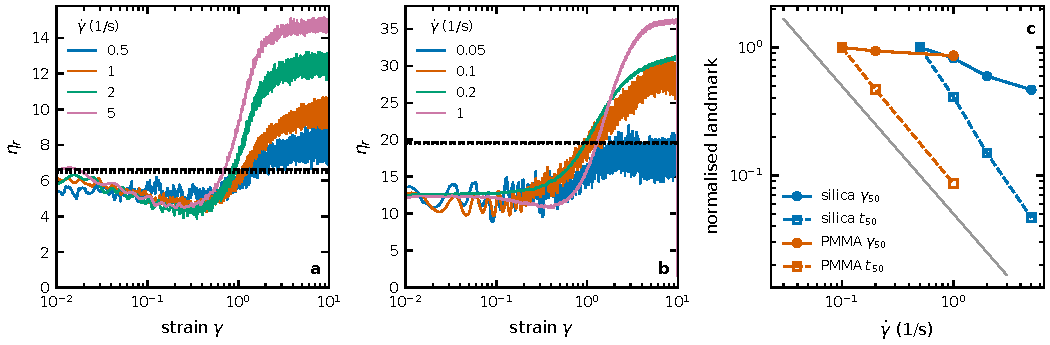
\includegraphics[width=\textwidth]{../figures/fig_reversal.pdf}
\caption{(a,b) Post-reversal relative viscosity against strain, from Ref.~\cite{Lin2015}:
(a) $2\,\mu$m silica, (b) $1.4\,\mu$m PMMA. One curve per shear rate. Dashed: the WC
frictionless floor $(1-\phi/\phi_0)^{-n}$ from the steady fit. Dotted: the lowest viscosity
on the same sample's steady sweep. (c) The fit-free half-recovery landmark read as a
strain ($\gamma_{50}$, filled) and as a time ($t_{50}=\gamma_{50}/\dot\gamma$, open), each
normalised by its value at the lowest admitted rate. The grey line has slope $-1$.}
\label{fig:reversal}
\end{figure*}

\emph{Recovery is strain-controlled.} Over a $\rateSpanSi\times$ span in rate, a pure strain clock
leaves $\gamma_{50}$ unchanged and a pure time clock leaves $t_{50}$ unchanged.
Measured spreads are $\gamma_{50}$: $\gFiftySpreadSi\times$ and $t_{50}$: $\tFiftySpreadSi\times$
for silica, and $\gFiftySpreadPm\times$ and $\tFiftySpreadPm\times$ for PMMA [Fig.~\ref{fig:reversal}(c)].

\emph{The clock is of order one.} Figure~\ref{fig:clock}(a) collects the estimates. The fitted
constant is $\fullLoSi$--$\fullHiSi$ (silica, $\nRatesSi$ rates) and $\fullLoPm$--$\fullHiPm$
(PMMA, $\nRatesPm$ rates). Truncating the fit at $\gamma=3$ moves it by at most $1.37\times$.  % 1.37x: scripts/gate_g11.py G11d 'worst 1.371x'
The landmark $\gamma_{50}$ is $\gFiftyLoSi$--$\gFiftyHiSi$ and $\gFiftyLoPm$--$\gFiftyHiPm$. Every estimate on
both materials exceeds $\solverGammaZero$ by at least $\minOverSolver\times$, and exceeds the
step-stress value $0.023$ by more than an order of magnitude. One PMMA record
($0.05$\,s$^{-1}$) is excluded: its fitted plateau in $f$ lies outside $[0,1]$. The model
has no state for it, so it cannot test the model. Its clock is still shown, in grey.

\emph{On silica the clock falls with rate.} The fitted constant falls monotonically by
$\fullFallSi\times$ across the four silica rates. In Eq.~(\ref{eq:relax}) the effective
constant is $1/\gamma_{\rm eff}=1/\gamma_0+1/(\dot\gamma t_r)$, which can only \emph{rise}
toward $\gamma_0$ with rate. No positive $t_r$ produces the silica trend; the straight-line
fit returns $t_r<0$. The trend survives the start ambiguity only in part. Over after-minimum starts the fall is at least $\fallLowerSi\times$, and the clocks at $0.5$, $1$ and $2$\,s$^{-1}$ stay strictly ordered, but the $2$ and $5$\,s$^{-1}$ ranges overlap. On PMMA the clocks are not monotone in rate, so there the test
cannot decide either way.

\emph{The recovery is not a single exponential.} A two-component description beats one
component decisively on the silica. Correcting for it reduces the rate trend from
$\twoClockMOne\times$ to $\twoClockMFour\times$ but does not remove it. These come from a joint fit on a finer binning, so its single-exponential value, $\twoClockMOne\times$, differs slightly from the $\fullFallSi\times$ above
(\texttt{scripts/probe\_two\_clock.py}). The decomposition itself is not robust to the fit window: the two
fitted clocks moved severalfold between windows (probe docstring), so we do not interpret them as two processes. Figure~\ref{fig:clock}(b) shows the
underlying shape. The rise is slow, then fast, where Eq.~(\ref{eq:relax}) is steepest at its
start.

\begin{figure}
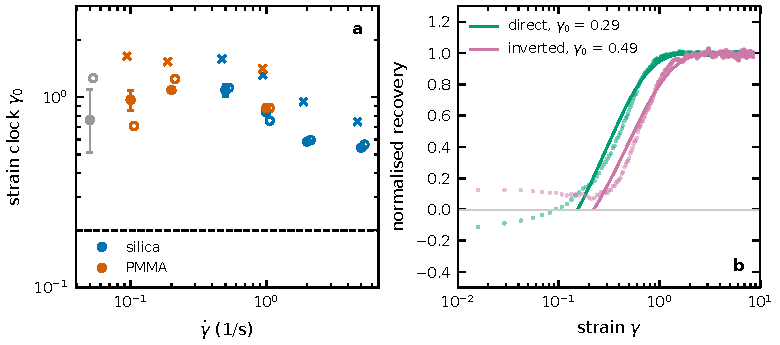
\includegraphics[width=\columnwidth]{../figures/fig_clock.pdf}
\caption{(a) The strain clock per shear rate: full-record fit in $f$ (filled, with its
profile interval), the same fit truncated at $\gamma=3$ (open), and the fit-free
$\gamma_{50}$ (crosses). Silica blue, PMMA orange; grey is the excluded PMMA record. The
dashed line is $\gamma_0=0.2$. (b) One simulated reversal from Ref.~\cite{Lin2015}
($\dot\gamma=0.74\dot\gamma_0$) read two ways, each normalised to its own fitted start and
plateau: the directly evaluated contact-stress fraction $s=\sigma_c/\sigma$, and the WC
inversion of the total viscosity. Lines are the fitted exponentials.}
\label{fig:clock}
\end{figure}

\emph{The clock depends on the definition of $f$.} Lin \emph{et al.}'s simulations report
the contact and hydrodynamic stresses separately. On that record the contact-stress fraction
$s=\sigma_c/\sigma$ can be fitted by the same code as the inverted $f$. The results are
$\gamma_0=\ctlDirect$ ($s$) and $\ctlInverted$ (inverted $f$), a $\ctlDiffPct\%$ difference
with non-overlapping intervals. The difference is identical at two packing triples
chosen so far apart that the inverted $f$ leaves $[0,1]$ in opposite directions. So it is the
inversion, not the gauge. WC's $f$ counts contacts, while $s$ is a fraction of stress, and nothing
requires them to be affinely related. They are not ($R^2=0.88$ between them).  % R2 0.88: scripts/probe_g11_direct_control.py 'affine to R2 = 0.8797'

\emph{A second protocol on silica: start-up is abrupt, not a relaxation.}
The deposit of \citet{Richards2019} contains constant-stress start-ups on a comparable
material: $4\,\mu$m silica in glycerol--water at $\phi=0.574$, with 17 steps of 20\,s,
each preceded by $\sim$14\,s at zero stress, and the same sample's steady curve. We
pre-registered the same fit (\texttt{PREREG\_startup\_clock\_2026-09-27.md}) and it
\emph{failed}. Above the onset ($\sigma\ge\suOnset$\,Pa) the fitted constants span
more than an order of magnitude across the steps, with $\chi^2_r$ up to $10^4$  % 0.027-0.885 (33x), chi2_r 73-11343: logs/probe_startup_clock.txt
 A single
exponential in strain does not describe these records, and the end-of-step viscosity also missed the steady curve by more than the registered $30\%$ at two stresses, so even the plateau being relaxed towards is not the steady one  % P3: worst 62%, at 3.0 and 9.5 Pa, logs/probe_startup_clock.txt
on this protocol. Figure~\ref{fig:startup}(a) shows
why. The viscosity does not relax. It stays near its low-stress value and then jumps
abruptly at $\gamma_j=\suJamLo$--$\suJamHi$ on all
$\suNAbove$ steps above onset. On $\suZeroCross$ of them the shear rate briefly reverses sign at $\gamma_j$. That is the rate ringing that gives Richards et al.'s paper its title~\cite{Richards2019}, a coupling of rheometer and sample, so those jumps are not a clean one-way material event. The fit-free reversal landmark $\gamma_{50}$ on Lin's
silica is at least $\reversalOverJam\times$ larger [Fig.~\ref{fig:startup}(b)]. The two
records are different samples, and we cannot tell whether $\gamma_j$ is a material strain
scale: over a $\suSigSpread\times$ range of stress it spreads $\suJamSpread\times$ in strain
and $\suTjSpread\times$ in time, so rotor spin-up is not excluded. A registered test that
$\gamma_j$ tracks the strain the sample recoils during the preceding rest also failed:
the recoil varies too little between steps to test it, although $\gamma_j$ exceeds it on
$\suJamAboveR$ above-onset steps (post hoc). What survives is qualitative. On silica, start-up produces an abrupt
rise in viscosity after a strain of order $0.1$, possibly coupled to the instrument. That is the scale reported for start-up
elsewhere~\cite{Richards2019,Han2018}, and it is not the order-one, gradual recovery that
reversal produces.

\begin{figure}
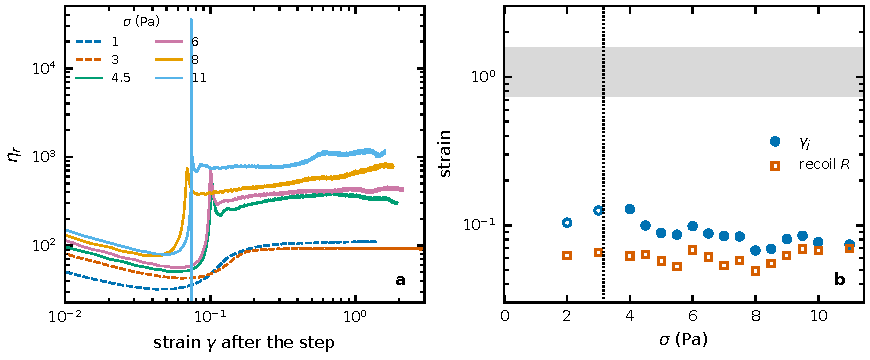
\includegraphics[width=\columnwidth]{../figures/fig_startup.pdf}
\caption{Constant-stress start-up on $4\,\mu$m silica in glycerol--water, $\phi=0.574$,
from the deposit of Ref.~\cite{Richards2019}. (a) Relative viscosity against strain after
the step, below (dashed) and above (solid) the steady thickening onset. The first
$\sim0.05$ in strain includes rotor spin-up. (b) The jam strain $\gamma_j$ (steepest fall
of the shear rate; filled above onset, open below) and the strain $R$ recovered during
the preceding rest, against stress. The dotted line marks the onset. The grey band is the
reversal half-recovery strain $\gamma_{50}$ on Lin's silica (Fig.~\ref{fig:reversal}),
for scale.}
\label{fig:startup}
\end{figure}

\begin{table*}
\caption{The Wyart--Cates strain clock by protocol. Literature values as stated in the
cited works (verified in \texttt{PRIOR\_ART\_STRAIN\_CLOCK\_2026-09-27.md}); ``this work''
values from \texttt{make\_numbers.py}.}
\label{tab:protocol}
\begin{ruledtabular}
\begin{tabular}{lll}
protocol & system & strain scale \\
\hline
step in stress & simulation & $0.023$~\cite{Mari2015} (used in~\cite{Chacko2018}) \\
imposed rate & corn starch & $O(10^{-1})$~\cite{Richards2019} \\
start-up (fronts) & corn starch & $\gamma^*\approx0.197$, other closure~\cite{Han2018} \\
start-up, constant $\sigma$ & $4\,\mu$m silica & abrupt at $\gamma_j=\suJamLo$--$\suJamHi$ (this work) \\
reversal & $2\,\mu$m silica & $\gamma_0=\fullLoSi$--$\fullHiSi$ (this work) \\
reversal & $1.4\,\mu$m PMMA & $\gamma_0=\fullLoPm$--$\fullHiPm$ (this work) \\
\end{tabular}
\end{ruledtabular}
\end{table*}

\section{Discussion}

Three statements survive every estimator we tried.
(i) Measured from reversal, the strain clock of scalar WC relaxation is of order one:
tens of times the step-stress value used in simulations, and several times
the start-up value from corn starch.
(ii) It is controlled by strain rather than time. On silica its rate dependence has the sign that
Eq.~(\ref{eq:relax}) with a time term forbids.
(iii) Reversal drives these suspensions below the model's frictionless floor. A scalar
$f$ can describe the recovery only after that state has been left.

Together with Table~\ref{tab:protocol}, these say that $\gamma_0$ is a property of a \emph{protocol and a definition},
not a material constant. Step, start-up and reversal probe different parts of the
microstructure's response. A scalar $f$ cannot distinguish them. The same record gives
clocks differing by $\ctlDiffPct\%$ depending on whether ``frictional fraction'' means a
contact count or a stress fraction. For solvers that run Eq.~(\ref{eq:relax}) in flows
containing reversal, such as drop impact, where the flow reverses at the rim, the
consequence is concrete. A clock taken from a step or a start-up is likely several times too
short for the recovery, and the softening immediately after reversal lies outside the
model's reach at any $\gamma_0$.

Limitations. Two materials from one laboratory for reversal, and a different sample for start-up, where instrument inertia is not excluded. The exponent $n$ is assumed; it matters at
the $2\%$ level. The single-exponential clock blends at least two processes. The
definition-dependence is measured on a simulation, not on the experiments. What is needed
next is reversal and step data on the same sample, with the contact contribution
measured directly (for example, by the method of Ref.~\cite{Lin2015}).

\emph{Data and code.} All numbers regenerate from \texttt{paper\_strain\_clock/make\_numbers.py}
and the figure scripts in the \texttt{dst\_fit} repository [URL to be added].

\bibliography{refs}

\end{document}
